%%%%%%%%%%%%%%%%%%%%%%%%%%%%%%%%%%%%%%%%%
% Beamer Presentation
% LaTeX Template
% Version 1.0 (10/11/12)
%
% This template has been downloaded from:
% http://www.LaTeXTemplates.com
%
% License:
% CC BY-NC-SA 3.0 (http://creativecommons.org/licenses/by-nc-sa/3.0/)
%
%%%%%%%%%%%%%%%%%%%%%%%%%%%%%%%%%%%%%%%%%

%----------------------------------------------------------------------------------------
%	PACKAGES AND THEMES
%----------------------------------------------------------------------------------------

\documentclass{beamer}

\mode<presentation> {

% The Beamer class comes with a number of default slide themes
% which change the colors and layouts of slides. Below this is a list
% of all the themes, uncomment each in turn to see what they look like.

%\usetheme{default}
%\usetheme{AnnArbor}
%\usetheme{Antibes}
%\usetheme{Bergen}
%\usetheme{Berkeley}
%\usetheme{Berlin}
%\usetheme{Boadilla}
%\usetheme{CambridgeUS}
%\usetheme{Copenhagen}
%\usetheme{Darmstadt}
%\usetheme{Dresden}
%\usetheme{Frankfurt}
%\usetheme{Goettingen}
%\usetheme{Hannover}
\usetheme{Ilmenau} % best so far
%\usetheme{JuanLesPins}
%\usetheme{Luebeck}
%\usetheme{Madrid}
%\usetheme{Malmoe}
%\usetheme{Marburg}
%\usetheme{Montpellier}
%\usetheme{PaloAlto}
%\usetheme{Pittsburgh}
%\usetheme{Rochester}
%\usetheme{Singapore}
%\usetheme{Szeged}
%\usetheme{Warsaw}

% As well as themes, the Beamer class has a number of color themes
% for any slide theme. Uncomment each of these in turn to see how it
% changes the colors of your current slide theme.

%\usecolortheme{albatross}
%\usecolortheme{beaver}
%\usecolortheme{beetle}
%\usecolortheme{crane}
%\usecolortheme{dolphin}
%\usecolortheme{dove}
%\usecolortheme{fly}
\usecolortheme{lily}
%\usecolortheme{orchid}
%\usecolortheme{rose}
%\usecolortheme{seagull}
%\usecolortheme{seahorse}
%\usecolortheme{whale}
%\usecolortheme{wolverine}

%\setbeamertemplate{footline} % To remove the footer line in all slides uncomment this line
\setbeamertemplate{footline}[page number] % To replace the footer line in all slides with a simple slide count uncomment this line
%\setbeamertemplate{frametitle continuation}[from second]

%\setbeamertemplate{navigation symbols}{} % To remove the navigation symbols from the bottom of all slides uncomment this line
}

\usepackage{graphicx} % Allows including images
\usepackage{booktabs} % Allows the use of \toprule, \midrule and \bottomrule in tables
\usepackage{csquotes}
\usepackage[font=tiny,labelfont=bf]{caption}
\usepackage{url}
\usepackage{qtree}
\usepackage{float}
\usepackage{tikz}
\usepackage{smartdiagram}
\usepackage{amsmath}
\usepackage{listings}

\usetikzlibrary{automata, positioning, arrows}
\usetikzlibrary{shapes.geometric,calc}

\graphicspath{{figures/}}

\bibliographystyle{plain}

% To quote
\let\oldquote\quote
\let\endoldquote\endquote
\renewenvironment{quote}[2][]
{\if\relax\detokenize{#1}\relax
	\def\quoteauthor{#2}%
	\else
	\def\quoteauthor{#2~---~#1}%
	\fi
	\oldquote}
{\par\nobreak\smallskip\hfill(\quoteauthor)%
	\endoldquote\addvspace{\bigskipamount}}

% To remove header
\makeatletter
\newenvironment{withoutheadline}{
	\setbeamertemplate{headline}[default]
	\def\beamer@entrycode{\vspace*{-\headheight}}
}{}
\makeatother

\setbeamercolor{block body alerted}{bg=alerted text.fg!10}
\setbeamercolor{block title alerted}{bg=alerted text.fg!20}
\setbeamercolor{block body}{bg=structure!10}
\setbeamercolor{block title}{bg=structure!20}
\setbeamercolor{block body example}{bg=green!10}
\setbeamercolor{block title example}{bg=green!20}

%\usepackage{natbib}
%\renewcommand\bibfont{\scriptsize}


%----------------------------------------------------------------------------------------
%	TITLE PAGE
%----------------------------------------------------------------------------------------

\title[Formalization]{Peter Naur's contribution to formal notations \\ and beyond} % The short title appears at the bottom of every slide, the full title is only on the title page

\author{Viktor Gsteiger} % Your name
\institute[unibas] % Your institution as it will appear on the bottom of every slide, may be shorthand to save space
{
University of Basel \\ % Your institution for the title page
\medskip
\textit{Seminar Turing Award Winners and Their Contributions} \\
\textit{v.gsteiger@unibas.ch} % Your email address
}
\date{November 26, 2020} % Date, can be changed to a custom date

\begin{document}
\begin{withoutheadline}
\begin{frame}
\titlepage % Print the title page as the first slide
\end{frame}
\end{withoutheadline}

\begin{withoutheadline}
\begin{frame}
	\frametitle{Formal notations in history}
	
	\begin{figure}
		\includegraphics[width=8cm]{1920px-Birch_bark_MS_from_Kashmir_of_the_Rupavatra_Wellcome_L0032691}
	\end{figure}
\end{frame}
\end{withoutheadline}

\begin{withoutheadline}
\begin{frame}
	\frametitle{New need for formal notations}
	
	\begin{figure}
		\includegraphics[width=8cm]{EDSAC_(19)}
	\end{figure}
\end{frame}
\end{withoutheadline}

\begin{withoutheadline}
	\begin{frame}
		\frametitle{Peter Naur}
		\begin{figure}
			\includegraphics[height=6cm]{Peternaur}
		\end{figure}
	\end{frame}
\end{withoutheadline}

\begin{withoutheadline}
	\begin{frame}
		\frametitle{Peter Naur's contribution}
		\begin{block}{Citation}
			For fundamental contributions to programming language design and the definition of Algol 60, to compiler design, and to the art and practice of computer programming.
	\end{block}
	\end{frame}
\end{withoutheadline}

%----------------------------------------------------------------------------------------
%	PRESENTATION SLIDES
%----------------------------------------------------------------------------------------

%------------------------------------------------
\section{Formal notations} % Sections can be created in order to organize your presentation into discrete blocks, all sections and subsections are automatically printed in the table of contents as an overview of the talk
%------------------------------------------------

\subsection{Phrase structure grammars}

\begin{frame}
	\frametitle{Phrase structure grammar}
	\begin{block}{Definition}
		Quadruple G = (V, $\Sigma$, P, S), where
		\begin{itemize}
			\item V is vocabulary
			\item $\Sigma$ $\subseteq$ V \textit{terminal symbols}
			\item S $\in$ (V - $\Sigma$) \textit{start symbol}
			\item P $\subseteq$ V*NV* $\times$ V* \textit{productions}
		\end{itemize}
	\end{block}
\end{frame}

\begin{frame}
	\frametitle{Phrase structure}
	\begin{exampleblock}{Example}
		\begin{equation*}
			\begin{aligned}
				G ={} ( & \{S, NP, VP, V, \text{the man}, \text{the book}, \text{took}\}, \\ 
				& \{\text{the man}, \text{the book}, \text{took}\}, P, S)
			\end{aligned}
		\end{equation*}
		\begin{equation*}
			\begin{split}
				P&: \\ S &\to NPVP \\
				VP &\to VNP \\
				NP &\to \text{the man} \\
				NP &\to \text{the book} \\
				V &\to \text{took}
			\end{split}
		\end{equation*}
	\end{exampleblock}
\end{frame}

\begin{frame}
	\frametitle{Chomsky Hierarchy}
	\begin{center}
		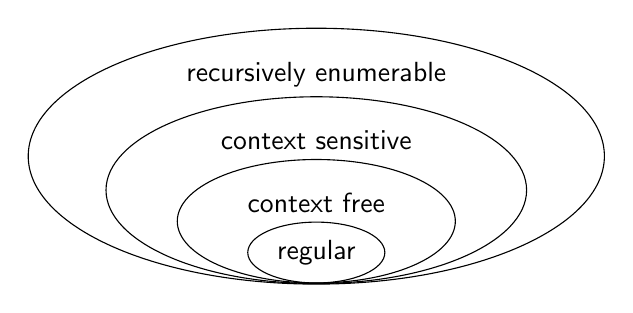
\begin{tikzpicture}[font=\sffamily,breathe dist/.initial=2ex]
		\foreach \X [count=\Y,remember=\Y as \LastY] in 
		{regular,context free,context sensitive,recursively enumerable}
		{\ifnum\Y=1
			\node[ellipse,draw,outer sep=0pt] (F-\Y) {\X};
			\else
			\node[anchor=south] (T-\Y) at (F-\LastY.north) {\X};
			\path let \p1=($([yshift=\pgfkeysvalueof{/tikz/breathe dist}]T-\Y.north)-(F-\LastY.south)$),
			\p2=($(F-1.east)-(F-1.west)$),\p3=($(F-1.north)-(F-1.south)$)
			in ($([yshift=\pgfkeysvalueof{/tikz/breathe dist}]T-\Y.north)!0.5!(F-\LastY.south)$) 
			node[minimum height=\y1,minimum width={\y1*\x2/\y3},
			draw,ellipse,inner sep=0pt] (F-\Y){};
			\fi}
		\end{tikzpicture}
	\end{center}
\end{frame}

\begin{frame}
\frametitle{Phrase structure in tree form}
	\begin{exampleblock}{Example}
		\begin{equation*}
			\Tree[.Sentence [.NP [ \textit{the man} ]]
					  [.VP [.Verb \textit{took} ]
							[.NP [.\textit{the book} ]]]]
		\end{equation*}
	\end{exampleblock}
\end{frame}

%------------------------------------------------

\subsection{Backus Naur form}

\begin{frame}
	\frametitle{Backus Normal form}
	\begin{exampleblock}{Example}
		\begin{equation*}
		\begin{split}
		<S> &:\equiv<NP>\text{ }<VP> \\
		<VP> &:\equiv<V>\text{ }<NP> \\
		<NP> &:\equiv\text{the man}\text{ }\textit{or}\text{ }\text{the book} \\
		<V> &:\equiv\text{took} \\
		\end{split}
		\end{equation*}
	\end{exampleblock}
\end{frame}

\begin{frame}
\frametitle{Backus Naur form}
	\begin{exampleblock}{Example}
		\begin{equation*}
			\begin{split}
				<sentence> &::=<noun\_phrase>\text{ }<verb\_phrase> \\
				<verb\_phrase> &::=<verb>\text{ }<noun\_phrase> \\
				<noun\_phrase> &::=\text{the man}\text{ }|\text{ }\text{the book} \\
				<verb> &::=\text{took} \\
			\end{split}
		\end{equation*}
	\end{exampleblock}
\end{frame}

%------------------------------------------------

\subsection{Programming languages, natural languages and mathematical languages}

\begin{frame}
\frametitle{Comparison of levels of formalization}
\begin{itemize}
	\item Natural languages
	\item Mathematical languages
	\item Programming languages
\end{itemize}
\end{frame}

\begin{frame}
	\frametitle{Language hierarchy}
	\begin{center}
		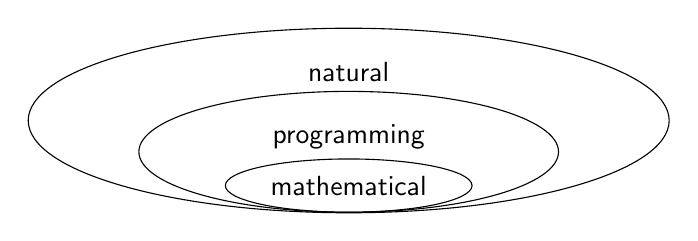
\begin{tikzpicture}[font=\sffamily,breathe dist/.initial=2ex]
		\foreach \X [count=\Y,remember=\Y as \LastY] in 
		{mathematical, programming, natural}
		{\ifnum\Y=1
			\node[ellipse,draw,outer sep=0pt] (F-\Y) {\X};
			\else
			\node[anchor=south] (T-\Y) at (F-\LastY.north) {\X};
			\path let \p1=($([yshift=\pgfkeysvalueof{/tikz/breathe dist}]T-\Y.north)-(F-\LastY.south)$),
			\p2=($(F-1.east)-(F-1.west)$),\p3=($(F-1.north)-(F-1.south)$)
			in ($([yshift=\pgfkeysvalueof{/tikz/breathe dist}]T-\Y.north)!0.5!(F-\LastY.south)$) 
			node[minimum height=\y1,minimum width={\y1*0.75*(\x2/\y3)},
			draw,ellipse,inner sep=0pt] (F-\Y){};
			\fi}
		\end{tikzpicture}
	\end{center}
\end{frame}

%------------------------------------------------
\section{Peter Naur's contribution}
%------------------------------------------------

\subsection{Algol in History}

\begin{frame}
\frametitle{Historical context}

\begin{center}
	\smartdiagramset{border color=none,
		set color list={blue!50!cyan,green!60!lime,orange!50!red,red!80!black},
		back arrow disabled=true}
	\smartdiagram[flow diagram:horizontal]{\tiny{FORTRAN},ALGOL 58,ALGOL 60,ALGOL 68}
\end{center}

\end{frame}

\begin{frame}
	\frametitle{Fortran}
	
	\begin{figure}
		\includegraphics[width=10cm]{FORTRAN_Example}
	\end{figure}
	
\end{frame}

\begin{frame}
	\frametitle{Algol 58}
	
	\begin{figure}
		\includegraphics[width=10cm]{ALGOL58_Example}
	\end{figure}
	
\end{frame}

\begin{frame}
	\frametitle{Algol 60}
	
	\begin{figure}
		\includegraphics[width=10cm]{ALGOL60_Example2}
		\includegraphics[width=10cm]{ALGOL60_Example} \\
		+ Additional examples, semantics and types
	\end{figure}
	
\end{frame}

\begin{frame}
	\frametitle{Algol 68}
	
	\begin{figure}
		\includegraphics[width=10cm]{ALGOL68_Example}
		\includegraphics[width=10cm]{ALGOL68_Example2}
	\end{figure}
	
\end{frame}

\subsection{Algol 60}

\begin{frame}
	\frametitle{Properties of Algol 60}
	
	\begin{itemize}
		\item Block scope
		\item Call-by-value, call-by-name and call-by-reference parameter passing
		\item Formal specification
		\item No I/O facilities
	\end{itemize}
	
\end{frame}

\begin{frame}[fragile]
	\frametitle{Block scope}
	\begin{exampleblock}{Example}
		\begin{lstlisting}
		begin
		    integer X;
		    X := 5;
		    begin
		        integer X, Y;
		        X := 4;
		        Y := 8;
		    end
		    print(X);
		    Y := 12;
		end;
		\end{lstlisting}
	\end{exampleblock}
\end{frame}

\begin{frame}[fragile]
	\frametitle{Call-by-value}
	\begin{itemize}
		\item Callee parameter Value of arguments given
		\item No modification of caller argument
	\end{itemize}
	
\end{frame}

\begin{frame}[fragile]
	\frametitle{Call-by-name}
	\begin{itemize}
		\item Pass thunk
		\item Similar to call-by-reference
		\item Parameter is passed without evaluation
	\end{itemize}
	
\end{frame}

\begin{frame}[fragile]
	\frametitle{Call-by-name}
	
	\begin{exampleblock}{Example}
		\begin{lstlisting}
		procedure swap (a, b);
		integer a, b, temp;
		begin
		    temp := a;
		    a := b;
		    b:= temp
		end;
		\end{lstlisting}
	\end{exampleblock}
\end{frame}

\begin{frame}[fragile]
	\frametitle{Call-by-name}
	
	\begin{exampleblock}{Example}
		swap(x, y):
		\begin{lstlisting}
		temp := x;
		x := y;
		y := temp
		\end{lstlisting}
		sqap(i, x[i]):
		\begin{lstlisting}
		temp := i;
		i := x[i];
		x[i] := temp
		\end{lstlisting}
	\end{exampleblock}
\end{frame}

\begin{frame}[fragile]
	\frametitle{I/O facilities}
	\begin{exampleblock}{Example}
		\begin{lstlisting}
		begin
		    print('Hello world!'); 
		    comment error!
		end;
		\end{lstlisting}
	\end{exampleblock}
\end{frame}

%------------------------------------------------

\subsection{Art and practice of computer programming}

\begin{frame} % Need to use the fragile option when verbatim is used in the slide
\frametitle{Programming as theory building}
	\begin{itemize}
		\item Source code contains theory
		\item Transfer theory to next programmer
		\item Theory should be observable
	\end{itemize}
\end{frame}

\begin{frame} % Need to use the fragile option when verbatim is used in the slide
	\frametitle{Role of formal descriptions}
	\begin{center}
		\smartdiagram[circular diagram:clockwise]{Knowledge,
			Theory, Documentation, Exchange}
	\end{center}
\end{frame}

%------------------------------------------------

\begin{frame} % Need to use the fragile option when verbatim is used in the slide
\frametitle{Problems of over-formalization}

\begin{itemize}
	\item Hard to exchange
	\item Prone to errors
	\item Goal in itself
	\item Disconnected from environment
\end{itemize}

\end{frame}

\section{Computing vs. Human Thinking}

%------------------------------------------------

\begin{frame} % Need to use the fragile option when verbatim is used in the slide
	\frametitle{Computing Versus Human Thinking}
	\begin{itemize}
		\item Description of computers
		\item Description of human thinking
	\end{itemize}
\end{frame}

%------------------------------------------------

\begin{frame}
	\frametitle{Discussion}
	\textbf{Do you think that human thinking will be formally describable?}
\end{frame}

%------------------------------------------------

\section{Conclusion}

\begin{frame}[fragile] % Need to use the fragile option when verbatim is used in the slide
	\frametitle{Importance of formal notation}
	\begin{quote}{Peter Naur}
			For achieving clarity any formal mode of expression should be used, not as a goal in itself, but wherever it appears to be helpful to authors and readers alike.
	\end{quote}
\end{frame}

%------------------------------------------------

%------------------------------------------------

\begin{frame}
	\Huge{\centerline{The End}}
\end{frame}

%----------------------------------------------------------------------------------------
\begin{frame}
	\frametitle{References}
	\footnotesize{
		\bibliography{references}
	}
\end{frame}

\end{document} 